\documentclass[a4paper,12pt]{article}
\usepackage[utf8]{inputenc}

% CIRCUITOS
\usepackage{tikz, tkz-euclide}
\usepackage[american]{circuitikz}
\usepackage{siunitx}
\usetikzlibrary{arrows}

%QUIMICA
\usepackage{chemfig,chemmacros}

\chemsetup[chemformula]{format=\sffamily}
\renewcommand*\printatom[1]{\ensuremath{\mathsf{#1}}}
\setatomsep{2em}
\setdoublesep{.6ex}
\setbondstyle{semithick}


\begin{document}
    
    \section{CIRCUITOS ELÉTRICOS}
    
    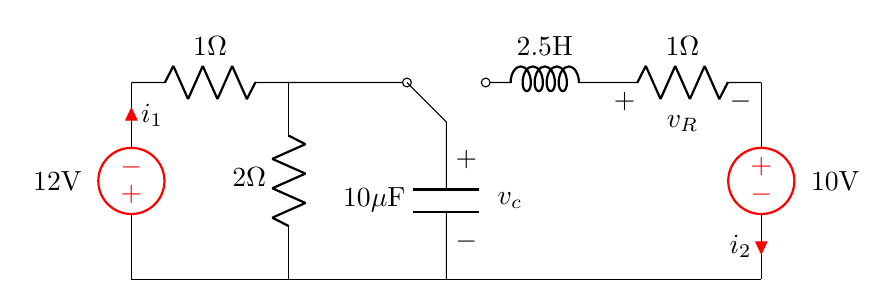
\begin{tikzpicture}
        \tkzDefPoints{  0  /0   /A,
                        0  /2.5 /B,
                        2  /2.5 /C,                        
                        3.5/2.5 /D,        
                        4.5/2.5 /E,        
                        6  /2.5 /F,
                        8  /2.5 /G,                        
                        8  /0   /H,
                        4  /0   /I,                        
                        2  /0   /J,
                        4  /2   /K}
                        

        \draw (A) to[V<=12V, i_=$i_1$,color=red] (B);
        
        \draw (B) to[R=\(\si{1\ohm}\)] (C);
        
        \draw (J) to[R=\(\si{2\ohm}\)] (C);
        
        \draw (C) to[short,-o] (D) to[open,-o] (E) to[cute inductor=2.5\si{\henry}] (F) to[R=\(\si{1\ohm}\),v>=\(v_R\)] (G);
        
        \draw (A) to (H);
        
        \draw (G) to[V<=10V, i_=$i_2$,color=red] (H);
        
        \draw (I) to[C=\(10\mu\si{\farad}\), v<=\(v_c\)] (K) to (D);
    
    \end{tikzpicture} \\
    
    \section{CIRCUITOS DIGITAIS}
    
    \begin{circuitikz} 
        \draw
          (0,2) node[nand port] (nand4) {}
          (2,3) node[nand port] (nand3) {}
          (4,2) node[nand port] (nand2) {}
          (0,0) node[nand port] (nand1) {}
          (nand1.out) |- (nand2.in 2)
          (nand4.out) |- (nand3.in 2)
          (nand3.out) |- (nand2.in 1)
          ;
        \draw 
            ([xshift=-1cm]nand1.in 1) 
              coordinate (aux) node[left] {$c$} to[short,*-] 
            (nand1.in 1);
        \draw 
            ([xshift=-1cm]nand1.in 2) 
                node[left] {$d$} to[short,*-] 
            (nand1.in 2);
        \draw 
            (aux|-nand3.in 1) 
                node[left] {$a$} to[short,*-] 
            (nand3.in 1);
        \draw
          (nand4.in 1) -- coordinate (middle) (nand4.in 2);
        \draw 
            (aux|-middle) 
                node[left] {$b$} to[short,*-]
            (middle);
        \end{circuitikz}
        
        \section{REAÇÕES QUÍMICAS}
        
        \begin{center}\small\setatomsep{1.5em}
        \schemestart
        \chemfig{*6(=-=(-(=[2]O)-[::-60]O-[0]O-[::30](=[2]O)-[::-60]*6(=-=-=-))-=-)}
        \arrow{->[$\Delta$]}
        2 \chemfig{*6(=-=(-(=[2]O)-[::-60]\lewis{0.,O})-=-)}
        \arrow
        2 \chemfig{*6(=-=(-[,.15,,,draw=none]\lewis{0.,})-=-)}\+\ch{2 CO2 ^}
        \schemestop
        \end{center}
\end{document}
